\documentclass[titlepage=firstiscover, bibliography=totoc, captions=tableheading]{scrartcl}
\title{V207: Das Kugelfall - Viskometer nach Höppler}
\author{
  Simon Schulte
  \texorpdfstring{
    \\
    \href{mailto:simon.schulte@udo.edu}{simon.schulte@udo.edu}
  }{}
  \texorpdfstring{\and}{, }
  Tim Sedlaczek
  \texorpdfstring{
    \\
    \href{mailto:tim.sedlaczek@udo.edu}{tim.sedlaczek@udo.edu}
  }{}
}
\publishers{TU Dortmund – Fakultät Physik}

\date{Durchführung: 15.11.2016\\
      Abgabe: 22.11.2016}

\usepackage[aux]{rerunfilecheck}
\usepackage{polyglossia}
\setmainlanguage{german}
\usepackage{amsmath}
\usepackage{amssymb}
\usepackage{mathtools}
\usepackage{fontspec}

\usepackage{scrhack}
\usepackage{float}
\floatplacement{table}{htbp}
\floatplacement{figure}{htbp}

\usepackage[locale=DE, separate-uncertainty=true, per-mode=symbol-or-fraction]{siunitx}
%\usepackage{siunitx}

\usepackage[style=alphabetic]{biblatex}
\addbibresource{lit.bib}

\usepackage[section, below]{placeins}
\usepackage[labelfont=bf,
font=small,
width=0.9\textwidth,
format=plain,
indention=1em]{caption}
\usepackage{graphicx}
\usepackage{grffile}
\usepackage{subcaption}

\usepackage[math-style=ISO, bold-style=ISO, sans-style=italic, nabla=upright, partial=upright]{unicode-math}
\setmathfont{Latin Modern Math}

\usepackage[autostyle]{csquotes}

\usepackage[unicode]{hyperref}

\usepackage{bookmark}

\usepackage{booktabs}

\usepackage[version=4, math-greek=default, text-greek=default,]{mhchem}

\begin{document}

\maketitle
\thispagestyle{empty}
\tableofcontents
\newpage

\section{Zielsetzung}
\label{sec:zielsetzung}
Es soll mit Hilfe der Kugelfallmethode bei einer laminaren Strömung die
Temperaturabhängigkeit der dynamischen Viskosität von destilliertem Wasser
bestimmt werden.

\section{Theorie}
\label{sec:theorie}
Wenn ein Körper sich durch eine Flüssigkeit bewegt, wirken, in entgegengesetzter
Richtung zur Gravitation Reibungskräfte. Diese hängen von der Fläche $A$, der Geschwindigkeit $v$
des Körpers und von der Viskosität $\eta$ der Flüssigkeit ab. Die Viskosität
einer Flüssigkeit hängt von der Temperatur ab. In diesem Versuch wird die
Viskosität von destilliertem Wasser untersucht, welche mit zunehmender
Temperatur geringer wird. Um besagte Viskosität zu bestimmen, lässt man eine
Kugel mit Radius $r$ laminar durch ein mit destilliertem Wasser gefülltes Rohr
fallen. Die Stokesche Reibung wird dann mit der Formel
\begin{equation}
  F_R = 6 \pi \eta v r
  \label{eqn:stokes}
\end{equation}
bestimmt, wobei $v$ die Fallgeschwindigkeit ist. Die Reibungskraft $\vec{F_R}$
und die Antriebskraft $\vec{F_A}$ wirken dabei der Gravitationskraft $\vec{F_g}$
entgegen. Die beiden entgegengesetzten Kräfte werden stärker, umso schneller
der Körper sich bewegt, solange, bis ein Kräftegleichgewicht entsteht und der
Körper eine konstante Geschwindigkeit erreicht. Dabei wird eine annäherend
laminare Strömung erzeugt. Indem man die Reynoldsche Zahl für die Bewegung
errechnet, lässt sich dann sagen, ob die Bewegung des Körpers tatsächlich
laminar war. Es gibt eine kritische Zahl für destilliertes Wasser, anhand
welcher man sehen kann, wenn die errechnete Reynoldsche Zahl kleiner oder größer
ist, ob die Bewegung laminar oder turbulent war. Um eine laminare Bewegung zu
gewährleisten, wird das Fallrohr um wenige Grade geneigt, sodass die Kugel an der
Rohrwand hinabgleitet und sich keine Wirbel ausbilden können. Der Durchmesser
des Körpers selbst ist nur geringfügig geringer, als der des Rohres. Mithilfe
der Dichte des destillierten Wassers $\rho_{Fl}$, der Dichte des Körpers $\rho_K$,
der Apperaturkonstante $K$ und der Fallzeit $t$ lässt sich dann die Viskosität
$\eta$ berechnen:
\begin{equation}
  \eta = K (\rho_K - \rho_{Fl}) \cdot t
  \label{eqn:dynVisk}
\end{equation}
Dabei enthält die Apperaturkonstante $K$ sowohl die Kugelgeometrie, als auch
die Fallhöhe. Da die Viskosität von vielen Flüssigkeiten stark
temperaturabhängig ist, wird die temperaturabhängige Viskosität durch die
Andradesche Gleichung:
\begin{equation}
  \eta(T) = A exp (\frac{B}{T})
  \label{eqn:dynViskvonT}
\end{equation}
beschrieben, mit den Konstanten A und B.

\section{Durchführung}
\label{sec:durchführung}
\subsection{Versuchsaufbau}
Wie in Abbildung 1 gezeigt fällt die Kugel durch ein Rohr, welches mit Wasser
gefüllt ist. Durch zwei Stopfen und jeweils einer Schraube über diesen Stopfen
an den beiden Rohrenden kann man sowohl Wasser, als auch die Kugel selbst, in das
Rohr füllen. An dem Rohr sind drei Messmarken befestigt, die jeweils mit einem
Abstand von $\SI{5}{\centi\meter}$ auseinander liegen. Diese werden zur Zeitmessung genutzt. Die
Libelle wird genutzt, um zu prüfen, ob das Viskosimeter gerade steht. Um die
Temperatur des Wassers im Rohr regulieren zu können, nutzt man ein Thermostat,
an welchem man die Temperatur des Wassers, welches das Rohr in einem
zylinderförmigen Körper umgibt, einstellen kann.
\begin{figure}[htb]
  \centering
  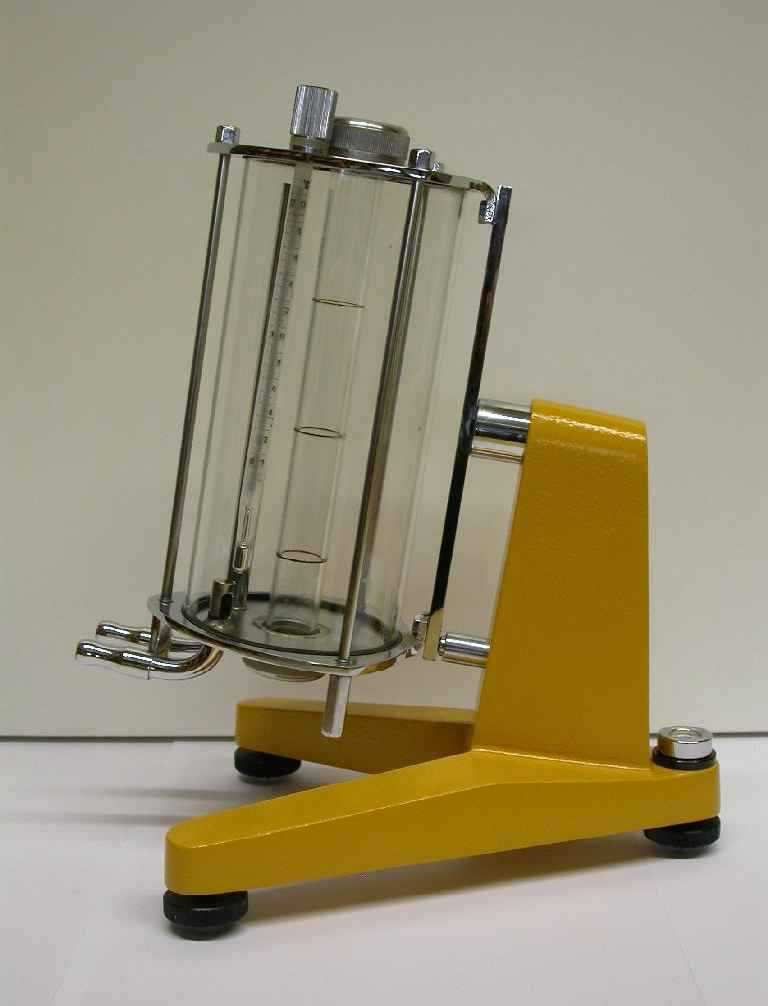
\includegraphics[width=0.5\textwidth]{figure/bild.png}
  \caption{Das Höppler - Viskometer}
  \label{fig:viskosimeter}
\end{figure}
\subsection{Versuchsdurchführung}
Zunächst bestimmt man die Masse und die geometrischen Maße der beiden Kugeln.
Dabei fällt auf, dass eine Kugel größer als die andere ist.
Daraufhin überprüft man mit Hilfe der Libelle, ob das Viskometer gerade steht.
Als nächstes füllt man das Rohr mit destilliertem Wasser und sorgt dafür, dass sich
möglichst keine Luftbläschen mehr am Rande des Rohres befinden. Dafür nutzt man
einen Glasstab. Dann gibt man vorsichtig die Kugel in das Rohr und achtet
darauf, dass auch an der Kugel möglichst keine Luftbläschen sind, denn diese
würden die Messungen verfälschen. Nun misst man die Zeit, die die beiden Kugeln
bei Zimmertemperatur brauchen, um $\SI{10}{\centi\meter}$ Strecke zurückzulegen, also von der
obersten Markierung zur untersten zu gelangen. Dabei ist auf den bereits in der
Theorie angesprochenen Kräfteausgleich zu achten. Die beiden Markierungen sind
bewusst nicht am oberen Rand des Rohres befestigt, damit die Kugel etwas Zeit
hat, um eine konstante Geschwindigkeit zu erreichen. Durch
das Drehen des Rohres um 180 grad kann man dann die nächste Messung durchführen.
Diese Messung führt man dann für beide Kugeln jeweils 10 mal durch und misst die
Zeit. Für die große Kugel muss dann noch die Apperaturkonstante K bestimmt
werden. Danach heizt man das Wasserbad, welches das Rohr umgibt auf. Man führt
jeweils vier Messungen für 10 verschiedene Temperaturen durch. Diese
befinden sich zwischen $\SI{25}{\celsius}$ und $\SI{70}{\celsius}$. Es werden die Zeiten für die größere
Kugel gemessen.
Zuletzt errechnet man die Reynoldsche Zahl für die gemessenen Daten und
überprüft, ob die Strömung laminar ist.
\newpage
\section{Auswertung}
\label{sec:auswertung}
Sämtliche Fehlerrechnungen in der Auswertung wurden mit den Python-Bibliotheken
Numpy und Uncertainties durchgeführt.
Diese nutzen folgende Formel für die Mittelwerte:
\begin{equation}
    \bar{x}=\frac{1}{n}\sum_{i=1}^n x_i
    \label{eqn:mittelwert}
\end{equation}
Der Standardfehler des Mittelwertes ergibt sich nach
\begin{equation}
    \mathup{\Delta}\bar{x}=\sqrt{\frac{1}{n(n-1)}\sum_{i=1}^n\left(x_i-\bar{x}\right)^2}.
    \label{eqn:stdfehler}
\end{equation}
Resultiert eine Größe über eine Gleichung aus mehreren anderen fehlerbehafteten Größen, so
berechnet sich der Gesamtfehler nach der Gaußschen Fehlerfortpflanzung zu
\begin{equation}
    \mathup{\Delta}f(x_1,x_2,...,x_n)=\sqrt{\left(\frac{\mathup{d}f}{\mathup{d}x_1}\mathup{\Delta}x_1\right)^2+\left(\frac{\mathup{d}f}{\mathup{d}x_2}\mathup{\Delta}x_2\right)^2+ \dotsb +\left(\frac{\mathup{d}f}{\mathup{d}x_n}\mathup{\Delta}x_n\right)^2}.
    \label{eqn:gauß}
\end{equation}
\subsection{Messwerte}
Für die beiden Kugeln wurden folgende Daten gemessen:
\begin{table}
  \centering
  \caption{Durchmesser und Masse}
  \label{tab:kugeldaten}
  \sisetup{table-format=2.2}
  \begin{tabular}{
    S
    @{${}\pm{}$}
    S[table-format=1.2]
    S[table-format=1.2]
    @{${}\pm{}$}
    S[table-format=1.2]
    S
    @{${}\pm{}$}
    S[table-format=1.2]
    S[table-format=1.2]
    @{${}\pm{}$}
    S[table-format=1.2]
    }
    \toprule
    \multicolumn{4}{c}{Kleine Kugel} & \multicolumn{4}{c}{Große Kugel}\\
    \multicolumn{2}{c}{$d_\text{kl} \,/\, \si{\milli\meter}$} &
    \multicolumn{2}{c}{$m_\text{kl} \,/\, \si{\gram}$} &
    \multicolumn{2}{c}{$d_\text{gr} \,/\, \si{\milli\meter}$} &
    \multicolumn{2}{c}{$m_\text{gr} \,/\, \si{\gram}$} \\
    \midrule
    15.64 & 0.05 & 4.46 & 0.01 & 15.82 & 0.05 & 4.60 & 0.01 \\
    \bottomrule
  \end{tabular}
\end{table}

\begin{table}
  \centering
  \caption{Zeiten für beide Kugeln bei Raumtemperatur ca. \SI{20}{\celsius}}
  \label{tab:zeitenraumtemperatur}
  \sisetup{table-format=2.2}
  \begin{tabular}{S S}
    \toprule
    {$t_\text{gr} \,/\, \si{\second}$} & {$t_\text{kl} \,/\, \si{\second}$} \\
    \midrule
    98.41 & 12.87 \\
    98.41 & 13.03 \\
    98.20 & 13.27 \\
    98.64 & 13.04 \\
    97.96 & 13.03 \\
    98.01 & 12.81 \\
    97.46 & 12.86 \\
    97.60 & 12.84 \\
    97.04 & 12.91 \\
    97.52 & 12.72 \\
    98.16 & 12.78 \\
    97.84 & 12.80 \\
    98.46 & 12.76 \\
    97.72 & 12.92 \\
    98.04 & 12.93 \\
    98.18 & 12.93 \\
    97.64 & 12.92 \\
    97.72 & 12.87 \\
    97.64 & 12.84 \\
    97.04 & 12.78 \\
    \bottomrule
  \end{tabular}
\end{table}

\begin{table}
  \centering
  \caption{Zeiten für die große Kugel bei der jeweiligen Temperatur}
  \label{tab:zeiten}
  \sisetup{table-format=2.2}
  \begin{tabular}{S S S S S S S S S S}
    \toprule
    {$t_\text{\SI{25}{\celsius}} \,/\, \si{\second}$} &
    {$t_\text{\SI{30}{\celsius}} \,/\, \si{\second}$} &
    {$t_\text{\SI{35}{\celsius}} \,/\, \si{\second}$} &
    {$t_\text{\SI{40}{\celsius}} \,/\, \si{\second}$} &
    {$t_\text{\SI{45}{\celsius}} \,/\, \si{\second}$} \\
    \midrule
    89.58 & 79.35 & 72.87 & 66.58 & 60.46 \\
    89.07 & 79.87 & 72.04 & 65.77 & 59.75 \\
    89.75 & 79.55 & 73.04 & 66.41 & 60.40 \\
    88.70 & 79.48 & 72.16 & 65.56 & 59.82 \\
    \bottomrule
  \end{tabular}
\end{table}
\begin{table}
  \centering
  \label{tab:zeiten}
  \sisetup{table-format=2.2}
  \begin{tabular}{S S S S S S S S S S}
    \toprule
    {$t_\text{\SI{50}{\celsius}} \,/\, \si{\second}$} &
    {$t_\text{\SI{55}{\celsius}} \,/\, \si{\second}$} &
    {$t_\text{\SI{60}{\celsius}} \,/\, \si{\second}$} &
    {$t_\text{\SI{65}{\celsius}} \,/\, \si{\second}$} &
    {$t_\text{\SI{70}{\celsius}} \,/\, \si{\second}$} \\
    \midrule
    55.03 & 50.63	& 47.10 & 43.12	& 40.63 \\
    54.80 & 50.33 & 46.66 & 43.03 & 40.69 \\
    55.12 & 50.80 & 47.33 & 43.35 & 40.44 \\
    54.33 & 50.15 & 46.50 & 43.15 & 40.41 \\
    \bottomrule
  \end{tabular}
\end{table}
\clearpage
\subsection{Bestimmung der Dichten}
Zu Beginn soll die Dichte der beiden Kugeln bestimmt werden.
Hierzu verwendet man die Masse und das Volumen der Kugel.
Die Formel für das Volumen einer Kugel ist:
\begin{equation}
  V = \frac{4}{3} \pi \left( \frac{d}{2} \right)^{\!\! 3}
  \label{eqn:volumen}
\end{equation}
Bei einer homogenen Massenverteilung folgt dann für die Dichte:
\begin{equation}
  \rho = \frac{m}{V}
  \label{eqn:dichte}
\end{equation}
Damit ergeben sich dann folgende Werte für die Dichten der beiden Kugeln:
\begin{table}
  \centering
  \label{tab:kugeldichten}
  \sisetup{table-format=1.2}
  \begin{tabular}{
    S
    @{${}\pm{}$}
    S
    S
    @{${}\pm{}$}
    S
    }
    \toprule
    \multicolumn{2}{c}{$\rho_\text{kl} \:/\: \si{\gram\per\cubic\centi\meter}$} &
    \multicolumn{2}{c}{$\rho_\text{gr} \:/\: \si{\gram\per\cubic\centi\meter}$} \\
    \midrule
    2.23 & 0.02 & 2.22 & 0.02 \\
    \bottomrule
  \end{tabular}
\end{table}

\subsection{Bestimmung der Konstante K der großen Kugel}
Um die in Formel \eqref{eqn:dynVisk} erwähnte Apparatekonstante K der großen Kugel zu bestimmen,
ermittelt man zunächst die beiden Mittelwerte der Fallzeiten bei Raumtemperatur.
Diese sind in der Tabelle \ref{tab:mittelfallzeitenraumT} dargestellt.
\begin{table}
  \centering
  \caption{Mittelwerte der Fallzeiten bei Raumtemperatur}
  \label{tab:mittelfallzeitenraumT}
  \sisetup{table-format=2.2}
  \begin{tabular}{
    S
    @{${}\pm{}$}
    S[table-format=1.2]
    S
    @{${}\pm{}$}
    S[table-format=1.2]
    }
    \toprule
    \multicolumn{2}{c}{$\bar{t}_\text{kl} \,/\, \si{\second}$} &
    \multicolumn{2}{c}{$\bar{t}_\text{gr} \,/\, \si{\second}$} \\
    \midrule
    12.90 & 0.03 & 97.88 & 0.10 \\
    \bottomrule
  \end{tabular}
\end{table}

\begin{table}
  \centering
  \caption{Dichte von Wasser bei der jeweiligen Temperatur nach \cite{UMaStFl}}
  \label{tab:dichteWasser}
  \sisetup{table-format=2.0}
  \begin{tabular}{S S[table-format=1.4]}
    \toprule
    {$T \,/\, \si{\celsius}$} &
    {$\rho_\text{\ce{H2O}} \:/\: \si{\gram\per\cubic\centi\meter}$} \\
    \midrule
    20 & 0.9982 \\
    25 & 0.9971 \\
    30 & 0.9957 \\
    35 & 0.9940 \\
    40 & 0.9932 \\
    45 & 0.9902 \\
    50 & 0.9880 \\
    55 & 0.9857 \\
    60 & 0.9832 \\
    65 & 0.9806 \\
    70 & 0.9778 \\
    \bottomrule
  \end{tabular}
\end{table}
Durch Einsetzen der oben angegebenen Dichte von Wasser, bei $\SI{20}{\celsius}$, und der anderen
Werte der kleinen Kugel in \eqref{eqn:dynVisk} erhält man die dynamische Viskosität $\eta$ von Wasser bei $\SI{20}{\celsius}$.
Die Apparatekonstante $K_\text{kl}$ war mit $K_\text{kl}=\SI{0.07640}{\milli\pascal\cubic\centi\meter\per\gram}$
gegeben.
Damit folgt: $\eta \left( \SI{20}{\celsius} \right)=\SI{1.21(2)e-2}{\gram\per\centi\meter\per\second}$.
Durch entsprechendes Umformen der Formel auf K und einsetzen der Werte der große Kugel
erhält man schließlich $K_\text{gr}$.\\
\\
$K_\text{gr}=\SI{0.01013(26)}{\milli\pascal\cubic\centi\meter\per\gram}$
\subsection{Verhalten von destiliertem Wasser in Abhängigkeit von der Temperatur}
Um das verhalten der dynamischen Viskosität von destiliertem Wasser in Abhängigkeit von der Temperatur
zu analysieren, mittelt man zuerst die Fallzeiten, die bei Temperaturen von $\SI{20}{\celsius}$ bis $\SI{70}{\celsius}$
in 5er Schritten gemessen wurden. Die Ergebnisse dazu stehen in Tabelle \ref{tab:fallzeitenMittelT}\\
\begin{table}
  \centering
  \caption{Gemittelte Fallzeit bei der jeweiligen Temperatur}
  \label{tab:fallzeitenMittelT}
  \sisetup{table-format=2.2}
  \begin{tabular}{S[table-format=2.0] S @{${}\pm{}$} S[table-format=1.2]}
    \toprule
    {$T \,/\, \si{\celsius}$} &
    \multicolumn{2}{c}{$\bar{t} \,/\, \si{\second}$} \\
    \midrule
    25 & 89.27 & 0.24 \\
    30 & 79.56 & 0.11 \\
    35 & 72.53 & 0.25 \\
    40 & 66.08 & 0.25 \\
    45 & 60.11 & 0.19 \\
    50 & 54.82 & 0.18 \\
    55 & 50.48 & 0.15 \\
    60 & 46.90 & 0.19 \\
    65 & 43.16 & 0.07 \\
    70 & 40.54 & 0.07 \\
    \bottomrule
  \end{tabular}
\end{table}
\clearpage
Durch Einsetzen in Formel \eqref{eqn:dynVisk} zusammen mit den Werten der großen Kugel
erhält man diese verschiedenen Werte von $\eta$:
\begin{table}
  \centering
  \caption{Dynamische Viskosität von dest. Wasser bei der jeweiligen Temperatur}
  \label{tab:dynamischeViskosT}
  \sisetup{table-format=1.5}
  \begin{tabular}{S[table-format=2.0] S @{${}\pm{}$} S}
    \toprule
    {$T \,/\, \si{\celsius}$} &
    \multicolumn{2}{c}{$\eta \left( T \right) \,/\, \si{\gram\per\centi\meter\per\second}$} \\
    \midrule
    20 & 0.01210 & 0.00022 \\
    25 & 0.01105 & 0.00020 \\
    30 & 0.00986 & 0.00018 \\
    35 & 0.00900 & 0.00017 \\
    40 & 0.00820 & 0.00015 \\
    45 & 0.00748 & 0.00014 \\
    50 & 0.00683 & 0.00013 \\
    55 & 0.00630 & 0.00012 \\
    60 & 0.00587 & 0.00011 \\
    65 & 0.00541 & 0.00010 \\
    70 & 0.00510 & 0.00009 \\
    \bottomrule
  \end{tabular}
\end{table}
\newpage
In dem folgenden Graphen wurden die errechneten Werte von $\eta$ logarythmiert gegen den Kehrwert der
jeweiligen Temperatur in $\SI{}{\kelvin}$ aufgetragen.
Außerdem wurde eine lineare Kurvenanpassung an die Andradesche Gleichung \eqref{eqn:dynViskvonT} durchgeführt
um die Parameter A und B zu ermitteln. M ist dabei die Steigung der Ausgleichsgeraden, sodass $A = e^M$.\\
$M=\SI{-10.44(5)}{}$\\
$A=\SI{2.9(1)e-5}{\gram\per\centi\meter\per\second}$\\
$B=\SI{1765(15)}{\kelvin}$

\begin{figure}
  \centering
  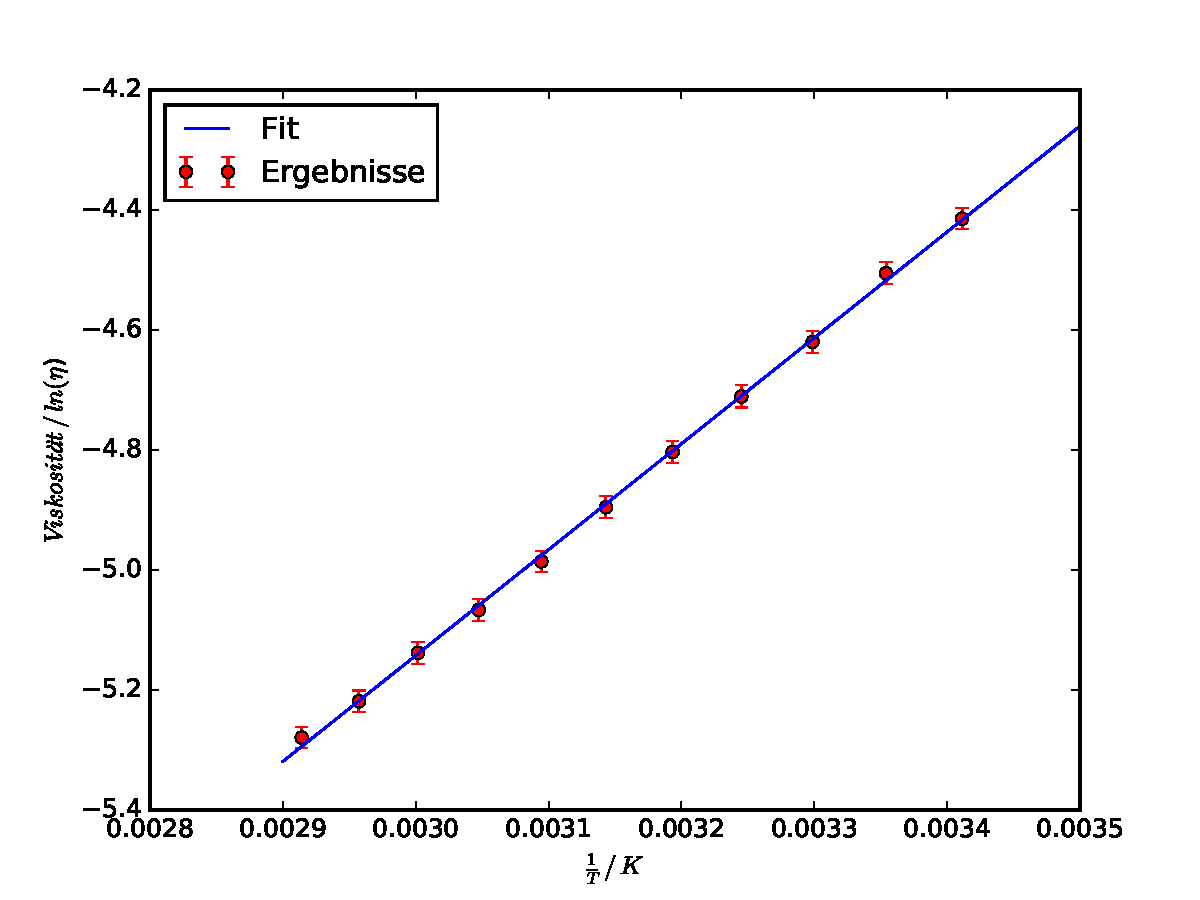
\includegraphics[width=\textwidth]{figure/Plot.pdf}
  \caption{Graph der gemessenen Werte von $\eta$ in Abhängigkeit von der Temperatur, mit Fit-Kurve.}
  \label{fig:plot}
\end{figure}
\newpage
\subsection{Theoretische Rechnung zur Andradesche Gleichung}
Um Vergleichswerte zu erhalten nutzen wir nun theoretische Werte für $\eta$ \ref{tab:dynamischeViskosTlit} und führen
erneut die Ausgleichsrechnung durch.
\begin{table}
  \centering
  \caption{Literaturwerte: Dynamische Viskosität von dest. Wasser bei der jeweiligen Temperatur \cite{UMaStFl}.}
  \label{tab:dynamischeViskosTlit}
  \sisetup{table-format=1.5}
  \begin{tabular}{S[table-format=2.0] S}
    \toprule
    {$T \,/\, \si{\celsius}$} & {$\eta \left( T \right) \,/\, \si{\gram\per\centi\meter\per\second}$} \\
    \midrule
    20 & 0.01002 \\
    25 & 0.00890 \\
    30 & 0.00798 \\
    35 & 0.00720 \\
    40 & 0.00653 \\
    45 & 0.00596 \\
    50 & 0.00547 \\
    55 & 0.00504 \\
    60 & 0.00467 \\
    65 & 0.00433 \\
    70 & 0.00404 \\
    \bottomrule
  \end{tabular}
\end{table}\\
Damit ergeben sich dann diese Werte für A und B:\\
$A=\SI{1.9(1)e-5}{\gram\per\centi\meter\per\second}$\\
$B=\SI{1821(22)}{\kelvin}$

\begin{figure}
  \centering
  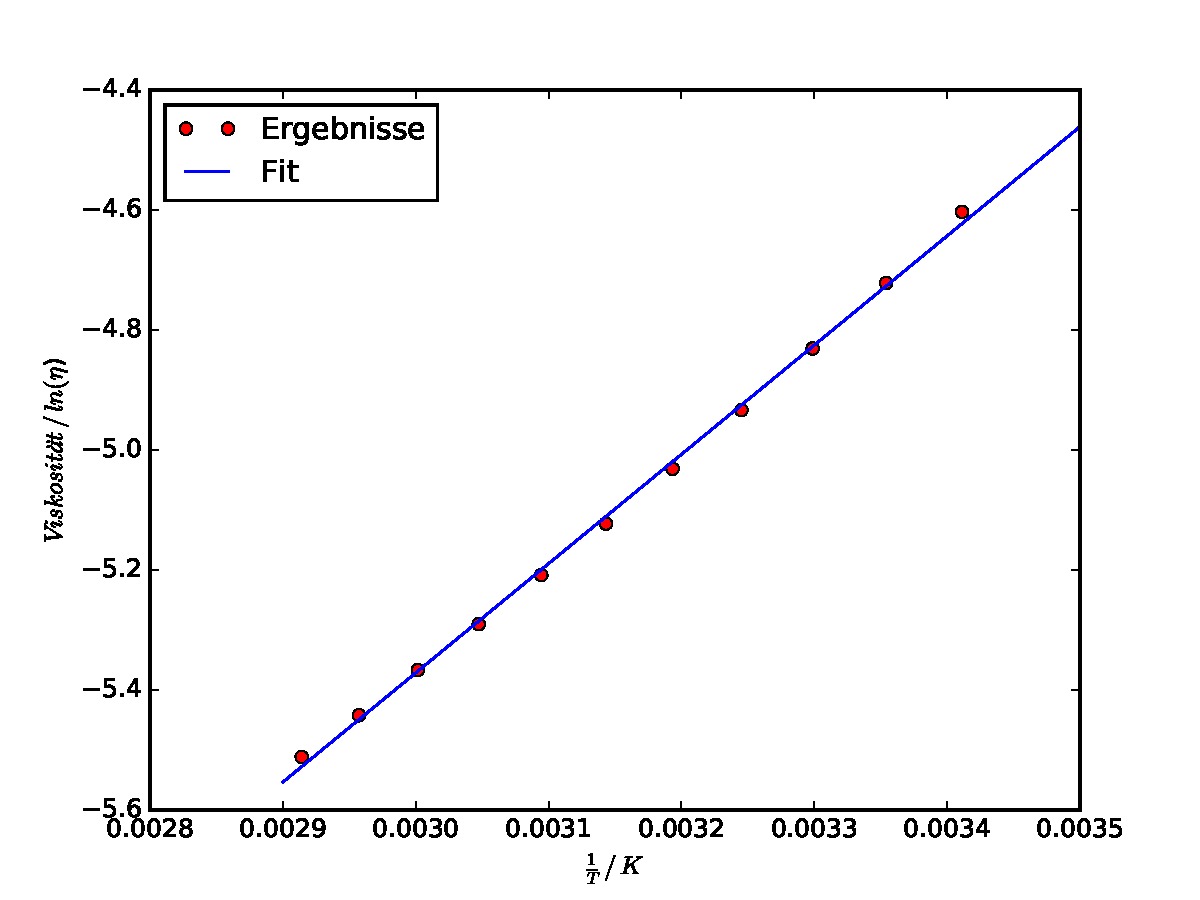
\includegraphics[width=\textwidth]{figure/Plot2.pdf}
  \caption{Graph der Literaturwerte von $\eta$ in Abhängigkeit von der Temperatur, mit Fit-Kurve.}
  \label{fig:plot2}
\end{figure}
\newpage
\subsection{Berechnung der Reynoldszahlen und Beurteilung ob die Strömung laminar ist}
Zur berechnung der Reynoldszahlen wird die Formel \cite{Maschbau}
\begin{equation}
  Re = \frac{\rho\cdot v \cdot d_\text{Kugel}}{\eta}
  \label{eqn:reynolds}
\end{equation}
verwendet. Dabei ist $\rho$ die Dichte des Wassers und $v$ die Geschwindigkeit der Kugel.
Mit dieser ergeben sich dann die folgenden Werte für die Reynoldszahlen:
\begin{table}
  \centering
  \caption{Reynoldszahlen der größeren Kugel bei der jeweiligen Temperatur}
  \label{tab:reynoldsgr}
  \sisetup{table-format=2.1}
  \begin{tabular}{S[table-format=2.0] S @{${}\pm{}$} S}
    \toprule
    {$T \,/\, \si{\celsius}$} &
    \multicolumn{2}{c}{$Re_\text{gr}$} \\
    \midrule
    20 & 13.3 & 0.2 \\
    25 & 16.0 & 0.3 \\
    30 & 20.1 & 0.4 \\
    35 & 24.1 & 0.5 \\
    40 & 29.0 & 0.6 \\
    45 & 34.8 & 0.7 \\
    50 & 41.7 & 0.8 \\
    55 & 49.0 & 0.9 \\
    60 & 56.5 & 1.1 \\
    65 & 66.4 & 1.2 \\
    70 & 74.9 & 1.4 \\
    \bottomrule
  \end{tabular}
\end{table}\\
Für die kleinere Kugel beträgt die Reynoldszahl\\
\\
$Re_\text{kl}=\num{100(2)}$\\
\\
Als Vergleichswert dient die kritische Reynoldszahl für eine Rohrströmung, welche 2300 beträgt \cite{Spektrum}.
Da unsere Reynoldszahlen viel kleiner sind handelt es sich bei der vorliegenden Strömung um eine laminare Strömung.
Das heißt, dass keine Turbulenzen entstehen.
\newpage
\section{Diskussion}
Der Versuch ist an einigen Stellen fehleranfällig: Die Temperatur ist nicht
immer perfekt konstant während der Zeitmessung, sondern verringert sich mit
der Zeit. Zudem wurde sie nur mit einem Thermometer gemessen und dafür keine Fehler
in betracht gezogen. Des Weiteren wurde die Zeit per Hand gemessen.
Die Literaturwerte, die zum Vergleich genutzt wurden, entsprechen der Dynamischen
Viskosität von Wasser bei $\SI{1}{\bar}$ Druck. In unserem Fall haben wir den Druck nicht
weiter berücksichtigt, was ebenfalls zu unterschieden führen kann.
Daraus resultierende Fehler sind jedoch nicht besonders groß, wie man an den
Ergebnissen sieht.
Die gemessenen Werte weichen nicht stark von den Literaturwerten ab
und die errechneten Reynoldzahlen lassen darauf schließen, dass wir in dem
Versuch eine laminare Strömung erzeugt haben.
Es ist sichtbar, dass sich die dynamische Viskosität von Wasser durch erhöhte
Temperaturen verkleinert.
\nocite{*}
\printbibliography

\end{document}
